\documentclass{beamer}
\usetheme{Madrid}

\title{Gate Problem on Control Systems}
\author{Aayush Goyal}
\centering
\date{IIT Hyderabad}
\begin{document}
\maketitle

\begin{frame}{Gate 2019 EC Problem}
\begin{flushleft}
    

\textsf{Q.6 - For an LTI system, the Bode plot for its gain is as illustrated in the figure shown. The number of system poles $N_{p}$ and number of system zeros $N_{z}$ in the frequency range 1 Hz $\leq$ f $\leq$ $10^{7}$ Hz is}
\end{flushleft}

\begin{figure}[htp]
    \centering
    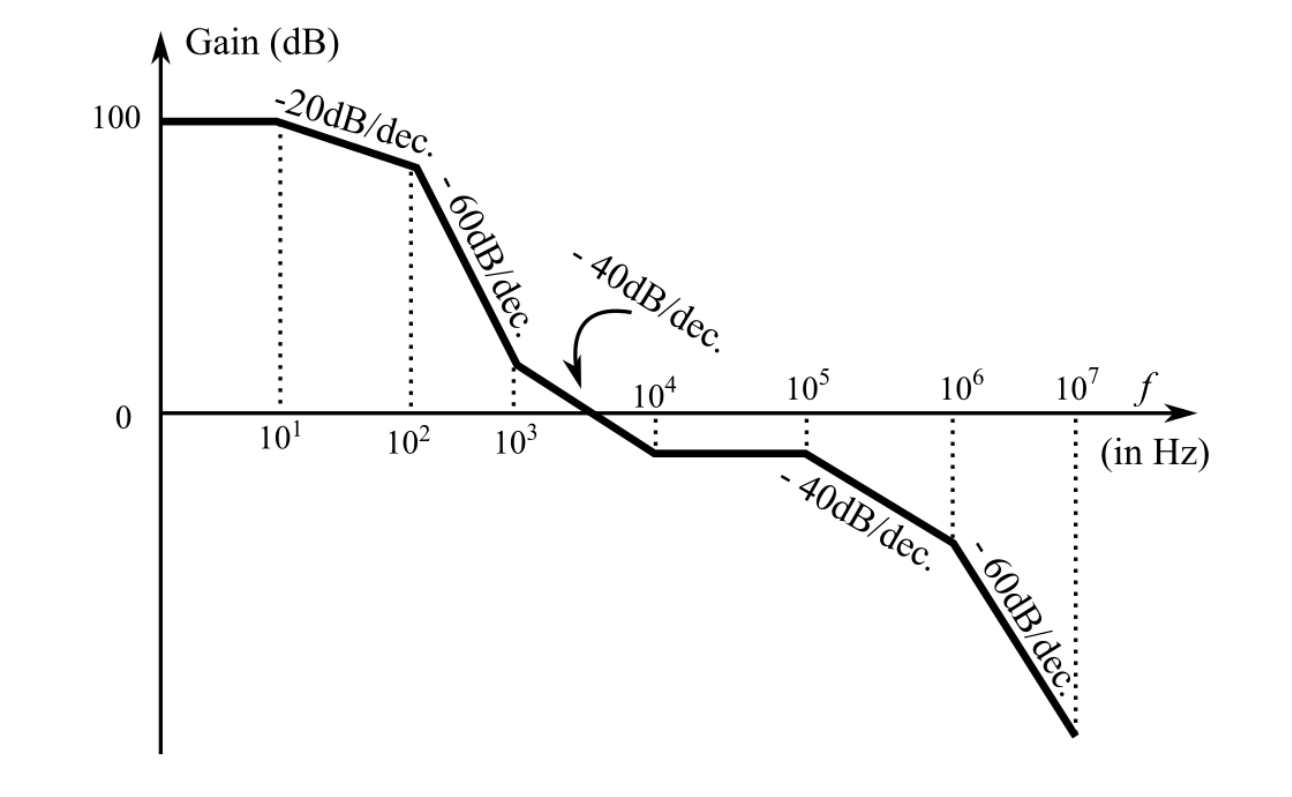
\includegraphics[width=9cm]{figure}
    
    \label{fig:galaxy}
\end{figure}
\end{frame}
\begin{frame}{Solution}
\begin{flushleft}
\textsf{Let us consider a generalized transfer gain}
\end{flushleft}
\vspace{10pt}
$H(s) = k \frac{(s-z_{1})(s-z_{2})...(s-z_{m-1})(s-z_{m})}{(s-p_{1})(s-p_{2})....(s-p_{n-1})(s-p_{n})}$\vspace{18pt}
$Gain = 20log|H(s)| = 20log|k| + 20log|s-z_{1}| + 20log|s-z_{2}| + ...... + 20log|s-z_{m}| - 20log|s-p_{1}| - 20log|s-p_{2}| - ..... - 20log|s-p_{n}| $ \vspace{18pt}

\begin{itemize}
    \item  When a pole is encountered the slope always decreases by -20 dB/decade
    \item When a zero is encountered the slope always increases by +20 dB/decade
\end{itemize}
\end{frame}

\begin{frame}{Solution}
  \begin{figure}[htp]
    \centering
    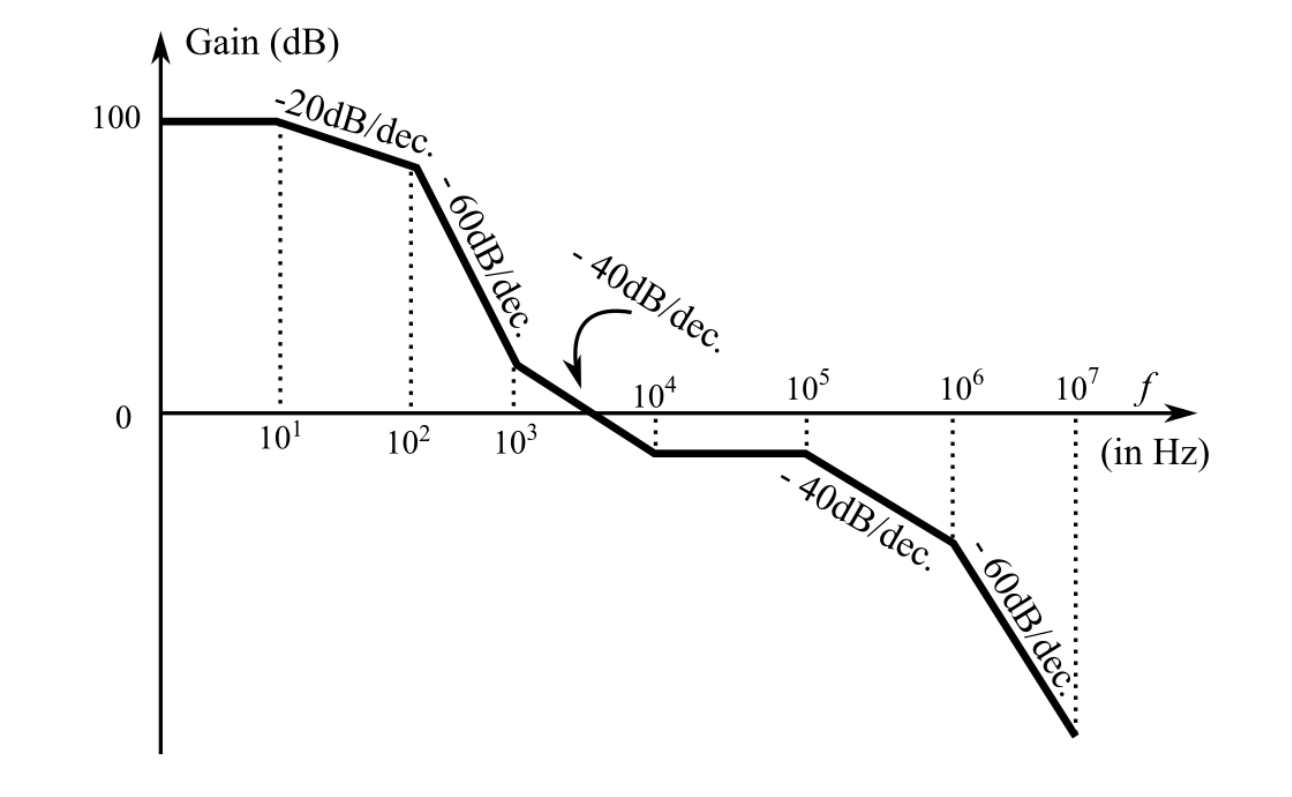
\includegraphics[width=7cm]{figure}
    
    \label{fig:galaxy}
\end{figure}
\begin{itemize}
    \item At f = 10 Hz , change in slope = -20dB/sec, Hence we have 1 pole here
    \item At f = $10^{2}$ Hz, Change in slope = -40dB/sec, Hence we have 2 poles here
    
    
    
\end{itemize}


\end{frame}
\begin{frame}{Solution}
  \begin{figure}[htp]
    \centering
    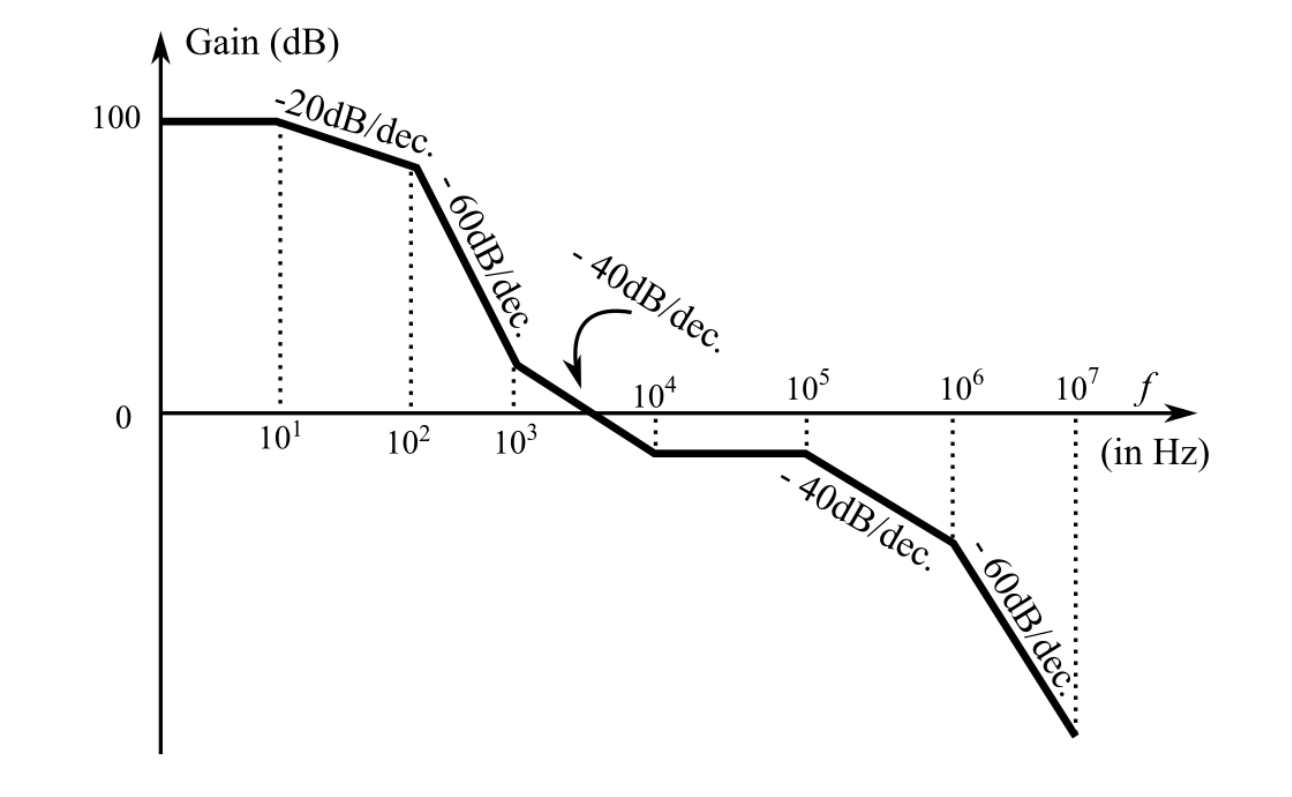
\includegraphics[width=7cm]{figure}
    
    \label{fig:galaxy}
\end{figure}
\begin{itemize}
\item At f = $10^{3}$ Hz, Change in slope = +20dB/sec, Hence we have 1 zero here
\item At f = $10^{4}$ Hz, Change in slope = +40dB/sec, Hence we have 2 zeros here

    
\end{itemize}


\end{frame}
\begin{frame}{Solution}
  \begin{figure}[htp]
    \centering
    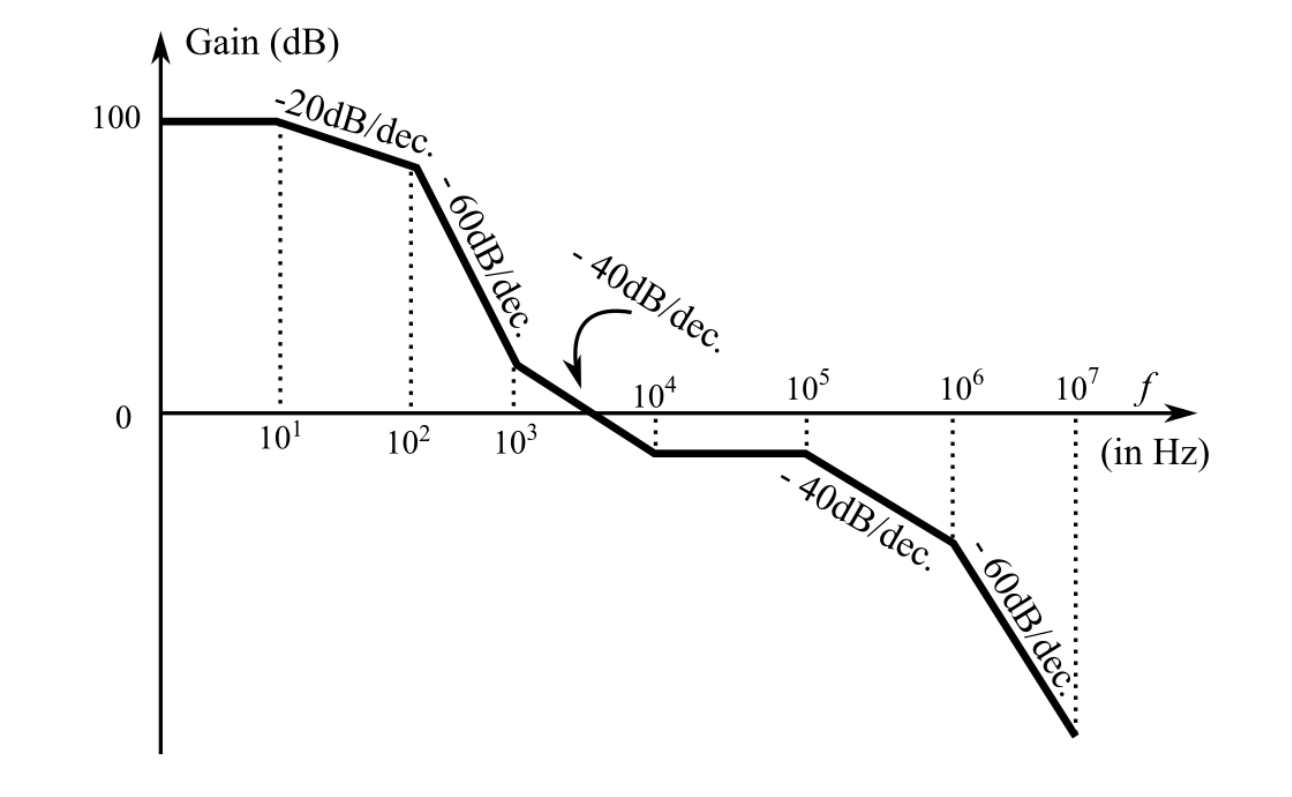
\includegraphics[width=7cm]{figure}
    
    \label{fig:galaxy}
\end{figure}
\begin{itemize}

    \item At f = $10^{5}$ Hz, Change in slope = -40dB/sec, Hence we have 2 poles here
    \item At f = $10^{6}$ Hz, Change in slope = -20dB/sec, Hence we have 1 pole here
    
\end{itemize}
\end{frame}
\begin{frame}{Answer}
\huge

$N_{p} = 6$ \linebreak
$N_{z} = 3$  



    
\end{frame}




\end{document}
